 \documentclass[a4paper,10pt]{article}
 \usepackage[utf8]{inputenc}  
 \usepackage[T1]{fontenc}
 \usepackage{graphicx}
 \graphicspath{{images/}} 
 
 \usepackage{wrapfig} 
 \usepackage{amsmath} 
 \usepackage{gensymb}
 \usepackage{fancyhdr}
 \usepackage{lastpage}
 \usepackage{textcomp}
 \usepackage{color}
 \usepackage{colortbl}
 \usepackage[table]{xcolor}
 \usepackage{courier}
 \usepackage{setspace}
 \usepackage{listings}
 \usepackage{ulem}%
 \usepackage{geometry}
 \usepackage{array}
 \usepackage{numprint}
 \usepackage{siunitx}
 \geometry{a4paper,
 total = {140mm, 237mm},
 left = 35mm,
 top = 30mm}
 \newcommand{\minus}{\scalebox{0.6}[1.0]{$-$}} 
 \newcommand{\signature}[2]{%
  \par\nobreak\bigskip
  \begin{singlespace}%
  \mbox{}\hfill\begin{tabular}{p{8cm} }
      \rule{8cm}{0.5pt}\newline{}%
        \textbf{#1}\\%
       #2 %
  \end{tabular}%
  \end{singlespace}%
  \medskip%
 }
 \pagestyle{fancy}
 \fancyhead[R]{Cellule déclenchement orage}
 \fancyfoot[C]{\thepage}
 \fancyhead[L]{Loïc Fracheboud}
 \author{Loïc Fracheboud}
 \title{Cellule déclenchement orage \\ Présentation \\ \Huge Storm Trigger}
 \date{29 juin 2016}
 \begin{document}
 \maketitle

 \begin{figure}[!h]
 \centering
 \vspace{80pt}
 
\includegraphics[scale=0.2]{images/signfracheboud}
 \end{figure}
 \pagebreak
 
 \section{Introduction}
  Le but de ce projet est de développer une cellule de déclenchement pour photographier les orages. Le concept est assez simple, il y a un capteur qui mesure la luminosité ambiante et un réglage qui permet de définir le seuil de déclenchement. Dès que le capteur détecte un changement de luminosité, un signal de déclenchement est envoyé à l'appareil photo connecté. \\

 \paragraph{Accessibilité}
 Dans l'idée de fournir une base ouverte, tout le travail est efectué avec des outils libres ou très courants, KiCAD pour la schématique/PCB, TexMaker pour la documentation, Github pour la gestion des versions, Excel pour les listes de matériel.
Le projet est disponible à l'adresse suivante : {\itshape https://github.com/loicfracheboud/StormTrigger}
  \begin{figure}[!h]
 \centering
 \vspace{5pt}
 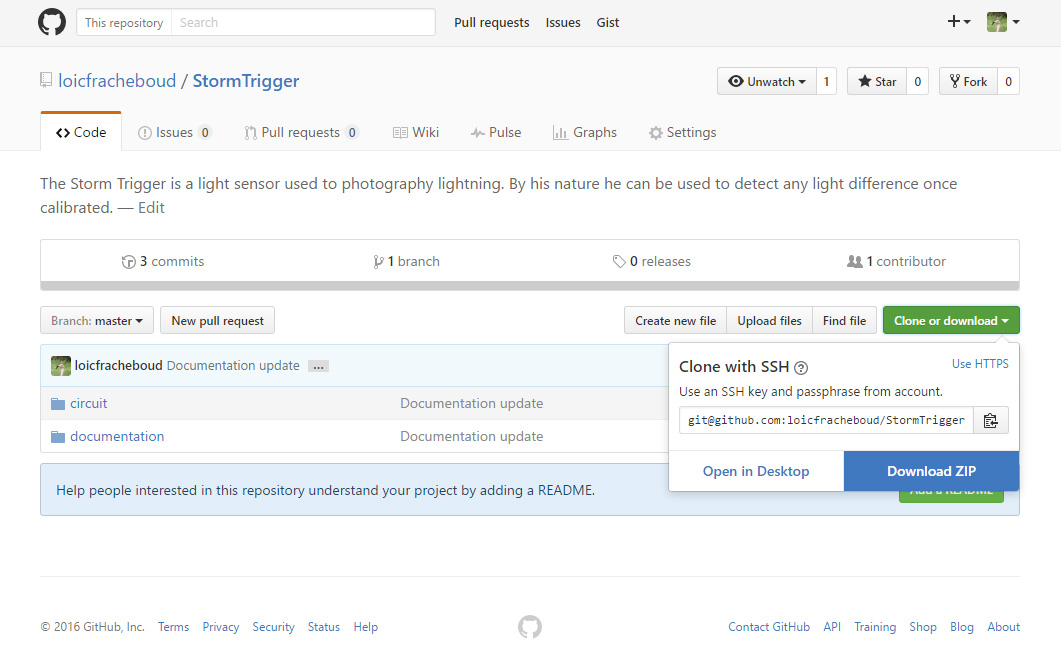
\includegraphics[scale=0.25]{images/git_dl}
 \caption{Cliquer sur "Download ZIP" pour avoir toute la documentation nécessaire}
 \end{figure}

  \section{Cahier des charges}
  Le cahier des charges a été établi selon les points suivants :
  \begin{enumerate}
    \item Déclenchement rapide
    \item Fonctionne sur piles/batteries AA
    \item Résiste à l'eau
    \item LED et buzzer pour indiquer le déclenchement, désactivables
    \item Compatible avec la plupart des appareils photos actuels
    \end{enumerate}
    
 \section{Conclusion}
  C'est un projet que j'ai eu en tête après une sortie de photo d'orage avec le groupe Passion Photographie. Par hasard deux jours après, je suis tombé sur Fabrice Giroud qui avait aussi dans l'idée de se faire une cellule. Du coup nous avons mis en place un petit groupe de réflexion pour définir les points importants du projet. Ce groupe est donc constitué de moi-même, Fabrice Giroud, Guillaume Schroeter, Mathieu Arlettaz, Emmanuel Boissard et Manoah Sauvin.\\
 
 \begin{wrapfigure}[0]{r}{6cm}
 \vspace{-52pt}
 \centering
 
\includegraphics[scale=1]{signfracheboud}
 \end{wrapfigure}
 \signature{Loïc Fracheboud}{Sion, le 19 juin 2016} 
 
  \begin{figure}[!h]
 \centering
 \vspace{100pt}
 
\includegraphics[scale=0.3]{images/signfracheboud}
 \end{figure}
 
 \pagebreak
 \section{Sources, liens divers}
 Dans cette section vous pourrez retrouver tous les liens importants du projet.
 
 \end{document}